\section{Proposed methodology}
\label{sec:methods}
In order to achieve our objectives we adopt and extend methods discussed in the literature review. These are explored further in the next sections.
\subsection{Objective 1}
Comprehensive multi modal sensor data collection for exercises is crucial if we are to address each research question mentioned above. As explored in the literature review, publicly available datasets for HAR and quality assessment seems to lack characteristics desirable to evaluate an end to end digital intervention. Therefore it is evident that there is a need for a dataset of multiple modalities with HAI for exercises. 
We propose a data collection task that will employ an array of sensor modalities with HAI.

\begin{figure}[ht]
\centering
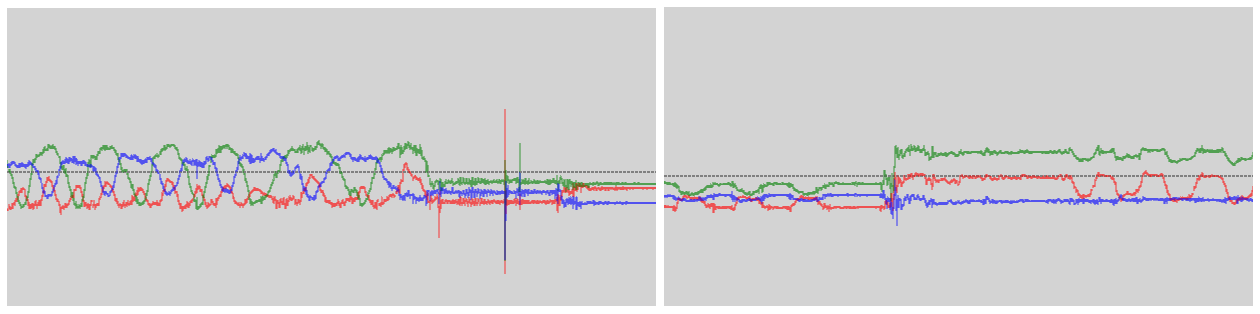
\includegraphics[width=0.8\textwidth]{acc}
\caption{Sample Accelerometer data}
\label {fig:acce}
\end{figure}

\begin{figure}[ht]
\centering
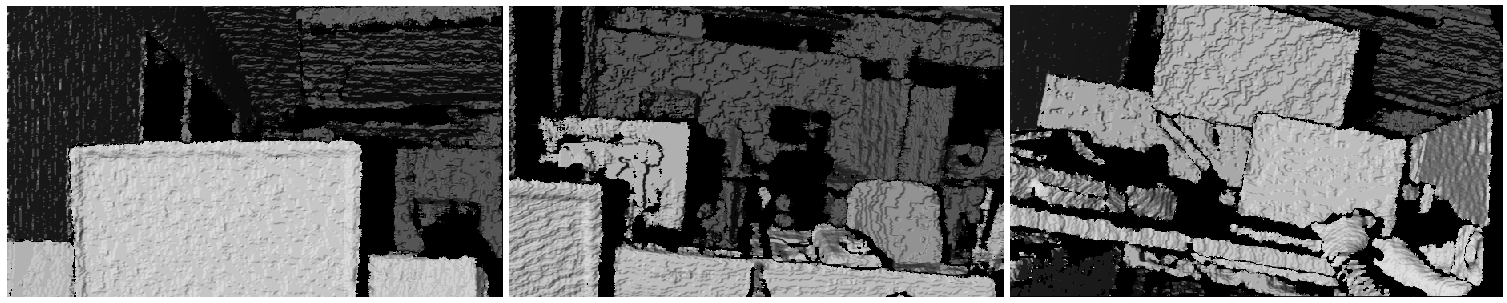
\includegraphics[width=0.8\textwidth]{dpt}
\caption{Sample Depth Camera data frames}
\label {fig:rgbd}
\end{figure}

Data collection will consist of two phases. First phase will focus on producing a multi-modal sensor dataset for exercise classification. We have selected accelerometers, pressure sensor and a depth sensor to bring together three different modalities. Figures \ref{fig:acce},\ref{fig:rgbd} and \ref{fig:pressure} show examples of these three modalities.

We have selected five exercises generally recommended for patients with low-back pain for this phase. Data will be recorded for thirty users each performing three sets of ten repetitions. A user will contribute roughly ten minutes of sensor data recordings and we will record approximately five hours of data distributed evenly across five classes. Data will be anonymized and analysed to remove outliers. This dataset will be used in design and evaluation of objectives 1 and 2.

\begin{figure}[ht]
\centering
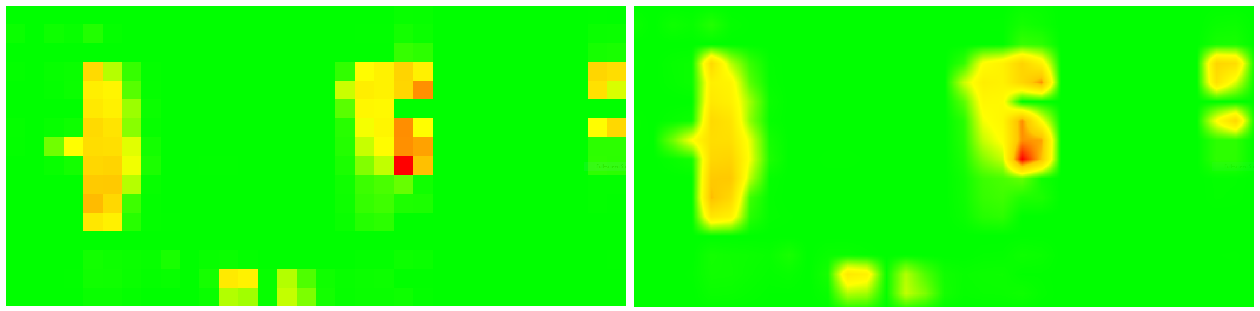
\includegraphics[width=0.8\textwidth]{pm}
\caption{Sample Pressure mat data frames, Left: Raw data frame (resolution 16x32), Right: Up-sampled with linear interpolation (resolution 512x1024) }
\label{fig:pressure}
\end{figure}

In phase two we will focus on producing a dataset with HAI by observing an exercise as a sequence of lower level actions. We will also create a test dataset with novice users to observe mistakes they do while performing the given exercises while labelling them on quality and on low level actions. The exercises and sensors selected for this phase will depend on conclusion we draw from objectives 1 and 2. 

\subsection{Objective 2}
To achieve objective 2 first we will investigate how each sensor modality contributes towards accurate classification of exercise movement classes and we will explore how a sensor fusion architecture can contribute toward improving previous results. Then we look at informed selection of sensors with an attention mechanism. Attention can be interpreted in different levels. First level is informed selection of subset of sensors for a given classification instance. At this level the goal is to select the best subset of sensors to intercept and recognise given an exercise. Second level is informed selection of features from abstract feature representations. We will generate feature embeddings at several abstract levels with a CNN for each modality and an attention mechanism focusing on the most desirable features from each sensor for the given classification instance. The goal is to attend to the most informative features from different sensors to improve exercise recognition.

\subsection{Objective 3}
Efficient deployment is an important characteristic in any health care digital interventions with direct impact on user acceptance. In this problem domain, the main restriction is the number of sensors. More sensors force the user in to a more restricted setting hence efficiency is negatively correlated to the number of sensors used. Being inspired by the PL paradigm we will explore two approaches to address objective 3. First is enforcing robustness in sensor fusion model to handle missing modalities. We will adapt the curriculum learning methodology to address this. We can define easy instances as instances where all modalities are present and hard instances as instances with some modalities missing and apply curriculum learning by introducing easy to hard instances in training phase. Second we will investigate how we can generate synthetic data to represent missing modalities at real time by adapting auto-encoders. At training auto-encoders can learn to generate sensor stream for each modality from other modalities, at test time auto encoder can be used to estimate the missing modality from existing. Thereafter the classifier will be presented with all modalities which will include both estimated and those actually present. We will conduct a comparative study to find the best approach. 

\subsection{Objective 4}
To address objective 4 we must define a metric to assess exercise performance quality.
Specifically the deviation between expected and actual performance will form the basis for this metric.
We will look at how deep models can learn differences in spatio-temporal data belonging to one classification class to evaluate quality difference. This will call for similarity measures in different abstract levels of feature embeddings. In order to locate differences in finer detail we will treat exercises as a sequence of primitive actions. Here the idea is to isolate the differences with respect to a primitive action rather than performing a binary evaluation. 

\subsection{Evaluation of Deep Models}
We will perform leave-one-user-out (LOUO) evaluation on deep models to evaluate model's ability to generalise across different users. Since qualitative assessment is largely user dependant, we will evaluate research question 3 with n-fold cross validation with personalized datasets. All deep architectures will be subjected to statistical significance test to evaluate how our methods compare with current state of the art.

\subsection{Dissemination}
Datasets will be published though UCI Machine Learning Repository \footnote{http://archive.ics.uci.edu/ml/index.php}. We will generate literature at each phase of the research and disseminate through conferences and workshops. All code will be made publicly available through git-hub \footnote{https://github.com}. We identify following deliverables for each objective listed in Section \ref{sec:research_questions}

\begin{outline}
\1 Objective 1 
\2 Phase 1 - Publish multi-modal exercises classification dataset.
\2 Phase 2 - Publish multi-modal HAI dataset for exercise quality evaluation 

\1 Objective 2 
\2 Publication on informed selection of sensors in fusion architectures for better performance.

\1 Objective 3 
\2 Publication on working with multi-modal fusion architecture in the absence of sensor modalities in real-time.

\1 Objective 4
\2 Publication on similarity comparison with deep architectures for spatio-temporal data

\2 Publication on exercise quality evaluation with HAI. 

\end{outline}